
\subsection{De la \english{partial reconfiguration} sur \virtex{}}

Devant l'impossibilité de faire de la \english{partial reconfiguration} sur Spartan6, une carte de développement dotée d'une \virtex{} nous a été fournie. Ce \fpga{} supporte bien la \english{partial reconfiguration} que ce soit en \english{difference-based} ou \english{module-based}. La solution était alors de garder le système sur la \nexys{} et de la faire communiquer avec la nouvelle carte.

\subsection{Communication entre la \virtex{} et la \nexys{}}

Après avoir examiné les possibilités que nous offraient les deux cartes, nous sommes partis sur l'idée de les faire communiquer via l'interface Ethernet. Évidemment, nous n'avions pas besoin de gérer toutes les fonctionnalités de la \english{link layer} comme définies dans le modèle OSI. Nous recherchions un moyen de communication qui s'occupe de l'accès au medium (CSMA/CD) ainsi qu'une certaine fiabilité des données transmises (CRC).\\
Du côté de la \nexys{}, une couche software s'occuperra de l'émission et de la transmission des données.\\
Sur la \virtex{} (voir figure \ref{virtex5-arch}), il n'y aura que des modules matériels communiquants entre eux :

\begin{itemize}
  \item un module Ethernet pour commmuniquer avec la \nexys{}.
  \item un bus de données Wishbone.
  \item de la RAM afin de stocker les données originales puis les données traitées par le module de PR.
  \item l'ICAP qui permettra de mettre en place le bitstream reçu via Ethernet.
  \item le module de PR qui effectuera les calculs sur les données.
  \item enfin, le module de contrôle du module de PR qui servira d'interface avec le bus et se chargera d'envoyer les données à traiter contenues en RAM vers le module de PR, puis de les récupérer pour les restocker en RAM. Lorsque l'opération sur les données sera finie, il renverra les résultats via l'Ethernet à la \nexys{}.
\end{itemize}

\begin{figure}[h!]
\centering
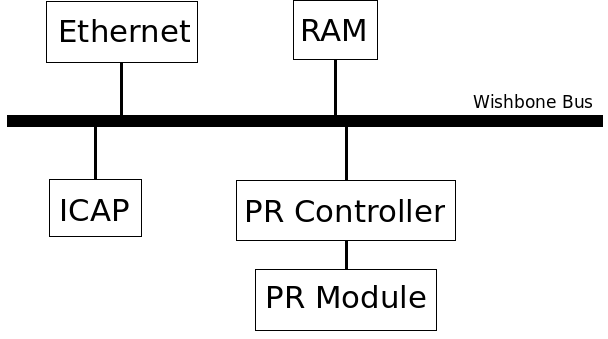
\includegraphics[scale=0.30]{virtex5-arch.png}
\caption{Schéma de l'architecture sur la carte pour le PR}
\label{virtex5-arch}
\end{figure}

\subsubsection{Protocole de communication}

Les échanges de données entre les deux cartes se feront au travers d'un protocole de communication simple. Les actions du côté de la \nexys{} sont illustrées par la figure \ref{nexys-side-protocol} et les actions du côté \virtex{} par la figure \ref{virtex-side-protocol}.\\
Partons de l'hypothèse que la Virtex5 et la \nexys{} sont dans l'état \textit{idle}. La \nexys{} enverra d'abord un ordre de reconfiguration à la Virtex5, puis le bitstream permettant d'effectuer le calcul. Ensuite la Virtex5 sera configurée et renverra un \textit{acknowkedgment} quand elle sera prête. La \nexys{} va alors envoyer les données à traiter puis se mettre en attente du résultat. Du côté de la \virtex{}, le calcul peut alors commencer. Une fois celui-ci fini, le contrôleur du module PR récupérera le résultat dans la RAM puis l'enverra via Ethernet à la \nexys{}.

\begin{figure}[h!]
\centering
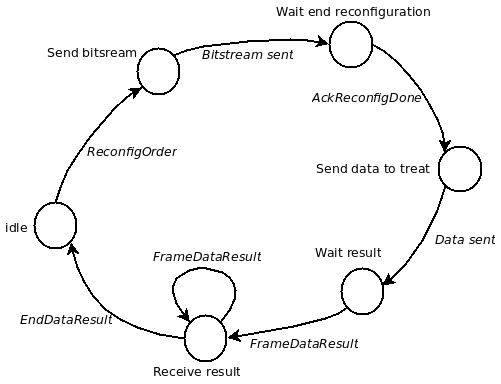
\includegraphics[scale=0.4]{nexys-side-protocol.png}
\caption{Protocole de communication du côté de la \nexys{}}
\label{nexys-side-protocol}
\end{figure}

\begin{figure}[h!]
\centering
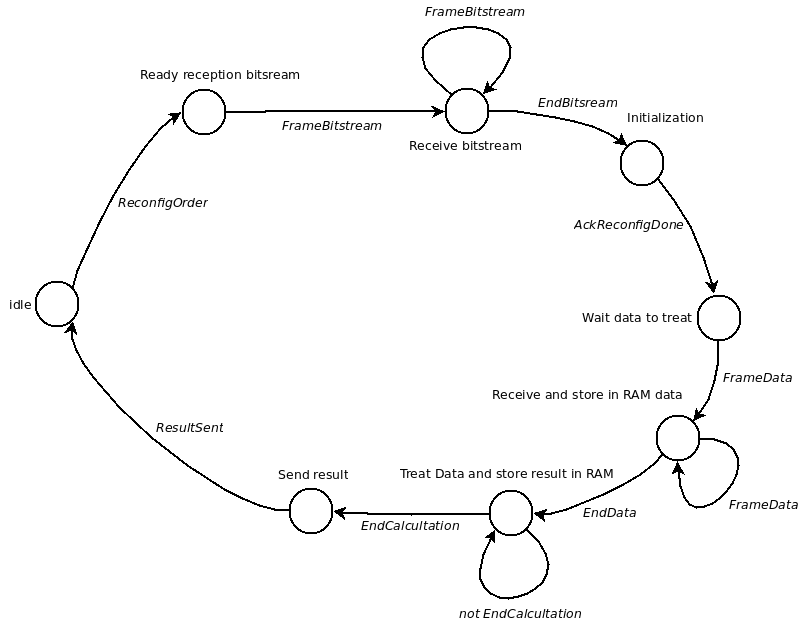
\includegraphics[scale=0.4]{virtex-side-protocol.png}
\caption{Protocole de communication du côté de la \virtex{}}
\label{virtex-side-protocol}
\end{figure}
